


  The length of each edge in the cube below is 2.
\begin{center}
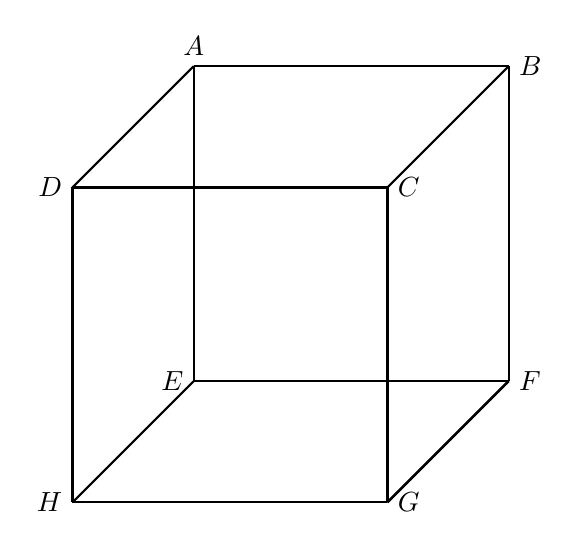
\begin{tikzpicture}
    \draw[thick] (0,0,0)--(0,0,4) node[left]{$H$};              
    \draw[thick] (0,4,4)--(0,0,4) ;              
  \draw[thick] (4,0,4)--(0,0,4) ;              

  \draw[thick] (0,0,0)--(0,4,0) node[above]{$A$};              
    \draw[thick] (0,4,4)--(0,4,0) ;              
  \draw[thick] (4,4,0)--(0,4,0) ;              




  \draw[thick] (4,0,0)--(0,0,0) node[left]{$E$};              
    \draw[thick] (4,0,4)--(4,0,0);              
  \draw[thick] (4,0,4)--(4,0,0) node[right]{$F$};              


   \draw[thick] (0,4,4)--(4,4,4) ;              
    \draw[thick] (4,4,4)--(4,0,4) node[right]{$G$};              
  \draw[thick] (4,4,4)--(0,4,4) node[left]{$D$};              
   \draw[thick] (4,4,0)--(4,4,4) node[right]{$C$};   
 \draw[thick] (4,0,0)--(4,4,0) node[right]{$B$};   

\end{tikzpicture}
\end{center}
What is the length of $\overline{AG}$ (not shown)? 



\ifsat
	\begin{enumerate}[label=\Alph*)]
		\item  $2$ 
		\item  $2\sqrt{3}$%
		\item  $2\sqrt{5}$
		\item  $4$
	\end{enumerate}
\else
\fi

\ifacteven
	\begin{enumerate}[label=\textbf{\Alph*.},itemsep=\fill,align=left]
		\setcounter{enumii}{5}
		\item  $2$ 
		\item  $2\sqrt{2}$  
		\item  $2\sqrt{3}$%
		\addtocounter{enumii}{1}
		\item  $2\sqrt{5}$
		\item  $4$
	\end{enumerate}
\else
\fi

\ifactodd
	\begin{enumerate}[label=\textbf{\Alph*.},itemsep=\fill,align=left]
		\item  $2$ 
		\item  $2\sqrt{2}$  
		\item  $2\sqrt{3}$%
		\item  $2\sqrt{5}$
		\item  $4$
	\end{enumerate}
\else
\fi

\ifgridin
  $2\sqrt{3}$%
		
\else
\fi

